
\documentclass{beamer}\usepackage[]{graphicx}\usepackage[]{color}
%% maxwidth is the original width if it is less than linewidth
%% otherwise use linewidth (to make sure the graphics do not exceed the margin)
\makeatletter
\def\maxwidth{ %
  \ifdim\Gin@nat@width>\linewidth
    \linewidth
  \else
    \Gin@nat@width
  \fi
}
\makeatother

\definecolor{fgcolor}{rgb}{0.345, 0.345, 0.345}
\newcommand{\hlnum}[1]{\textcolor[rgb]{0.686,0.059,0.569}{#1}}%
\newcommand{\hlstr}[1]{\textcolor[rgb]{0.192,0.494,0.8}{#1}}%
\newcommand{\hlcom}[1]{\textcolor[rgb]{0.678,0.584,0.686}{\textit{#1}}}%
\newcommand{\hlopt}[1]{\textcolor[rgb]{0,0,0}{#1}}%
\newcommand{\hlstd}[1]{\textcolor[rgb]{0.345,0.345,0.345}{#1}}%
\newcommand{\hlkwa}[1]{\textcolor[rgb]{0.161,0.373,0.58}{\textbf{#1}}}%
\newcommand{\hlkwb}[1]{\textcolor[rgb]{0.69,0.353,0.396}{#1}}%
\newcommand{\hlkwc}[1]{\textcolor[rgb]{0.333,0.667,0.333}{#1}}%
\newcommand{\hlkwd}[1]{\textcolor[rgb]{0.737,0.353,0.396}{\textbf{#1}}}%

\usepackage{framed}
\makeatletter
\newenvironment{kframe}{%
 \def\at@end@of@kframe{}%
 \ifinner\ifhmode%
  \def\at@end@of@kframe{\end{minipage}}%
  \begin{minipage}{\columnwidth}%
 \fi\fi%
 \def\FrameCommand##1{\hskip\@totalleftmargin \hskip-\fboxsep
 \colorbox{shadecolor}{##1}\hskip-\fboxsep
     % There is no \\@totalrightmargin, so:
     \hskip-\linewidth \hskip-\@totalleftmargin \hskip\columnwidth}%
 \MakeFramed {\advance\hsize-\width
   \@totalleftmargin\z@ \linewidth\hsize
   \@setminipage}}%
 {\par\unskip\endMakeFramed%
 \at@end@of@kframe}
\makeatother

\definecolor{shadecolor}{rgb}{.97, .97, .97}
\definecolor{messagecolor}{rgb}{0, 0, 0}
\definecolor{warningcolor}{rgb}{1, 0, 1}
\definecolor{errorcolor}{rgb}{1, 0, 0}
\newenvironment{knitrout}{}{} % an empty environment to be redefined in TeX

\usepackage{alltt}

\mode<presentation> {
\usetheme{Rochester}
\usecolortheme{seahorse}
}

\usepackage{graphicx} % Allows including images
\usepackage{booktabs} % Allows the use of \toprule, \midrule and \bottomrule in tables


\title{What is Beamer?} 

\author{Erin Kreiling} 
\institute[ASU]
{
Appalachian State University\\ 
\medskip
\textit{kreilingeg@email.appstate.edu} 
}
\date{\today}
\IfFileExists{upquote.sty}{\usepackage{upquote}}{} 

\begin{document}

\begin{frame}
\titlepage 
\end{frame}

\begin{frame}
\frametitle{Introduction} 
Creating a beamer class document really isn't very hard at all once you learn the basics! It has so many different features and you can put just about anything you want into a presentation! 
\end{frame}


\begin{frame}
\frametitle{How to Begin With Beamer}
\begin{figure}[ht!]
\centering
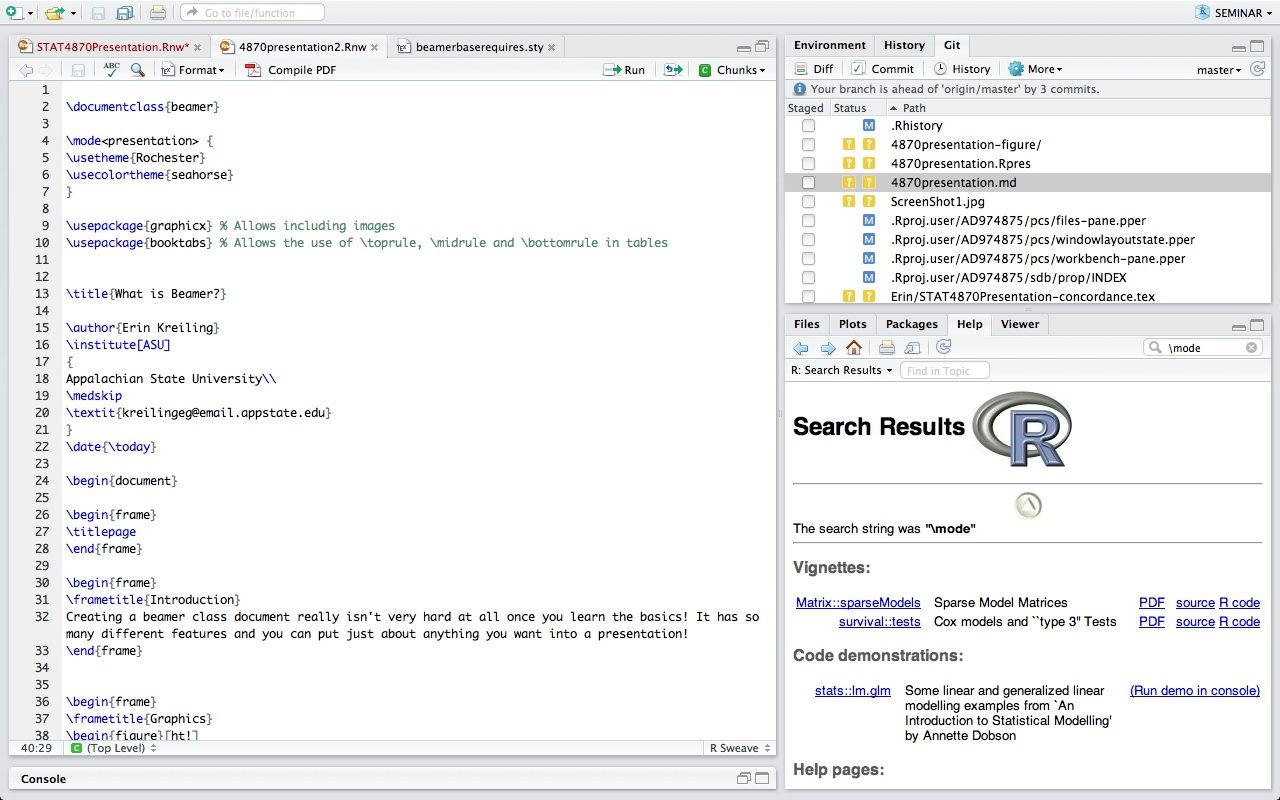
\includegraphics[width=90mm]{FinalScreenshot}
\end{figure}
\end{frame}

\begin{frame}
\frametitle{What Can Beamer Do For You?}
\begin{itemize}
\item
\newtheorem{thm}{The Central Limit Theorem}
\newtheorem{rmk}{The Fundamental Question of Inference}
\begin{thm}
If a sample is sufficiently large, then the distribution is approximately normal and the sample mean will be approximately equal to the population mean.
\end{thm}
\item
\begin{rmk}
How does what we observe compare to what would actually happen if the null hypothesis were true and we repeated the test over and over?
\end{rmk}
\end{itemize}
\end{frame}

\begin{frame}
\frametitle{How To Set Up Lists and Special Commands like Theorems}
\begin{figure}[ht!]
\centering
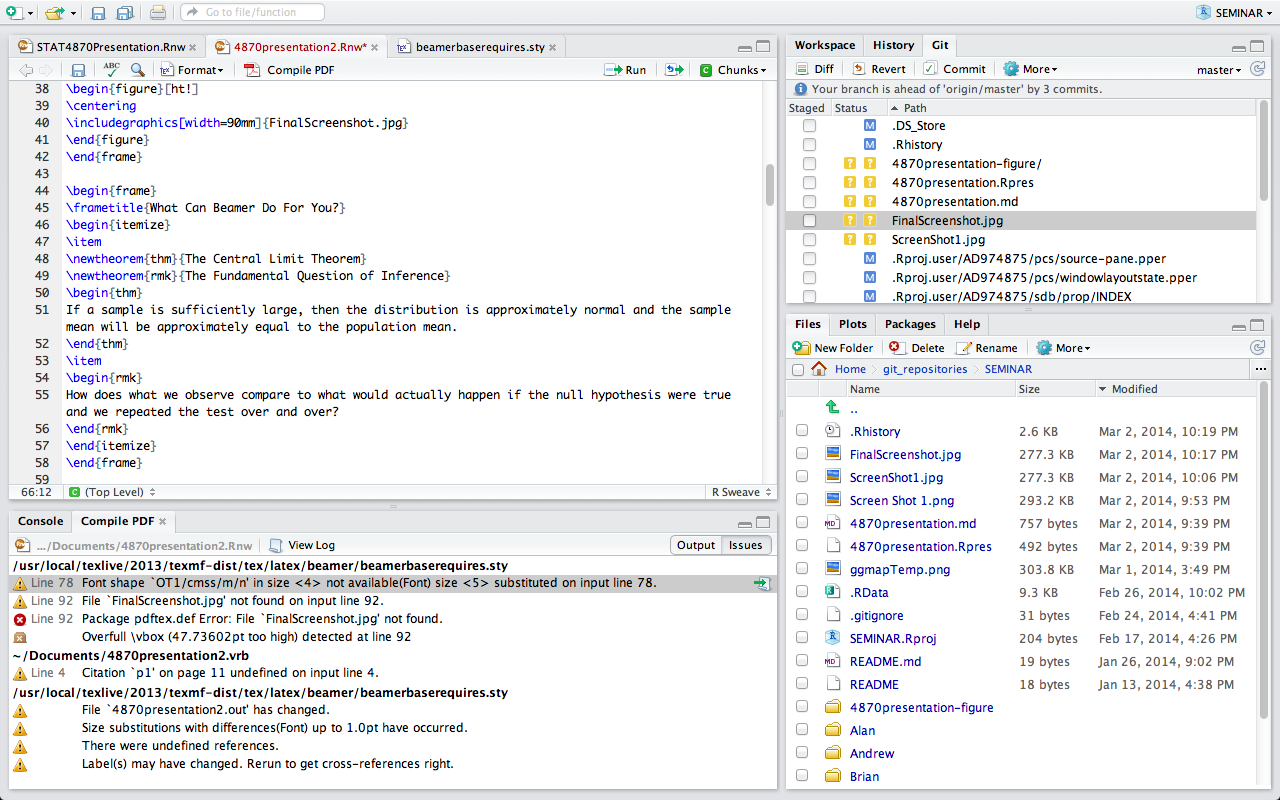
\includegraphics[width=90mm]{Screenshot02}
\end{figure}
\end{frame}

\begin{frame}
\frametitle{Other Options in Beamer}
\begin{itemize}
\item
\begin{definition}
         A \alert{prime number} is a number that has exactly two divisors.
       \end{definition}
\item
 \begin{itemize}
       \item 2 is prime (two divisors: 1 and 2).
         \pause
       \item 3 is prime (two divisors: 1 and 3).
         \pause
       \item 4 is not prime (\alert{three} divisors: 1, 2, and 4).
       \end{itemize}
  \begin{block}{Answered Questions}
    How many primes are there?
  \end{block}
  \begin{block}{Open Questions}
    Is every even number the sum of two primes?
  \end{block}
\end{itemize}
\end{frame}


\begin{frame}
\frametitle{Explanation}
\begin{figure}[ht!]
\centering
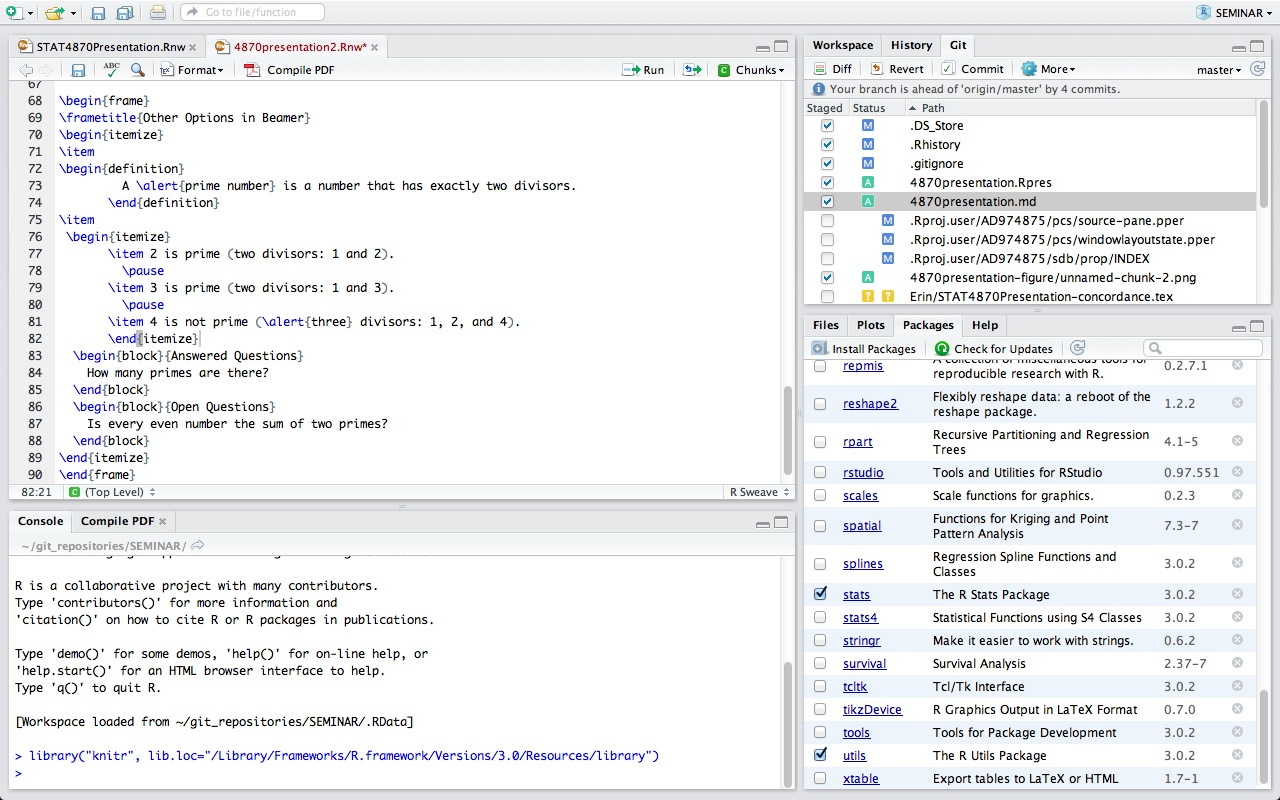
\includegraphics[width=90mm]{Screenshot03}
\end{figure}
\end{frame}

\end{document}
